\uuid{EXyV}
\chapitre{Série de Fourier}
\niveau{L2}
\module{Analyse}
\sousChapitre{Calcul de coefficients}
\titre{Fonctions périodiques et coefficients de Fourier}
\theme{séries de Fourier}
\auteur{}
\datecreate{2024-06-13}
\organisation{AMSCC}
\contenu{

\texte{ On considère les fonctions $f$ et $g$ comme dessinées ci-dessous, que l'on étend à des fonctions de $\R$ dans $\R$ qui sont impaires et $2\pi$-périodiques. 

\begin{center}
	\begin{tikzpicture}
		\begin{axis}[
			width=5cm, height=4cm,
			axis x line=center, xlabel={$x$},
			axis y line=middle, 
			%axis equal,
			legend style={draw=none,at={(1,1)},anchor=north west },
			samples=100,
			ymin=-1, ymax=3,
			xmin=-1, xmax=8,
			xtick={
				0 ,
				3, 7
			},
			xticklabels={
				$0$, $\frac{\pi}{k_0}$,$\pi$     },
			ytick={2},
			yticklabels={1 }
			]
			\addplot [mark=none, very thick, red,domain=0:3] {2};
			\addplot [mark=none, very thick, red,domain=3:7] {0};
			\legend{$f$ },
		\end{axis}
	\end{tikzpicture}
	\hspace{8em}
	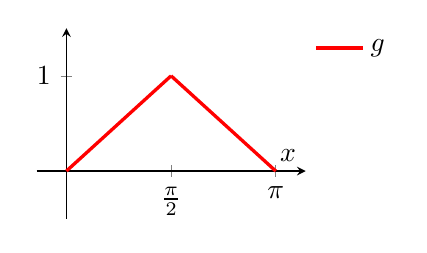
\begin{tikzpicture}
		\begin{axis}[
			width=5cm, height=4cm,
			axis x line=center, xlabel={$x$},
			axis y line=middle, 
			%axis equal,
			legend style={draw=none,at={(1,1)},anchor=north west },
			samples=100,
			ymin=-1, ymax=3,
			xmin=-1, xmax=8,
			xtick={
				0 ,
				3.5, 7
			},
			xticklabels={
				$0$, $\frac{\pi}{2}$,$\pi$     },
			ytick={2},
			yticklabels={1}
			]
			\addplot [mark=none, very thick, red,domain=0:3.5] {x*2/3.5};
			\addplot [mark=none, very thick, red,domain=3.5:7] {4-2*x/3.5};
			\legend{$g$ },
		\end{axis}
	\end{tikzpicture}
\end{center}
}

\begin{enumerate}
	\item \question{ Soit un entier $k_0 \geq 2$. Donner l'expression de $f(x)$ et de $g(x)$ en fonction de $x\in[0;\pi]$. }
	\reponse{On définit :
		$$f \colon x \mapsto \begin{cases}
			1&\text{si $x \leq \frac{\pi}{k_0}$}\\
			0&\text{si $x > \frac{\pi}{k_0}$}
		\end{cases}	\quad \text{et} \quad g \colon x \mapsto \begin{cases}
			\frac{2x}{\pi}&\text{si $x \leq  \frac{\pi}{2}$}\\
			2 - \frac{2x}{\pi} &\text{si $x > \frac{\pi}{2}$}
		\end{cases} $$
	}
	\item \question{ Calculer les coefficients de Fourier de $f$ puis exprimer la série de Fourier de $f$. }
	\reponse{La fonction $f$ étant impaire, les coefficients de Fourier $a_n(f)$ sont nuls et : 
		\begin{align*}
			b_n(f) &= \frac{2}{\pi} \int_0^{\pi} f(t)\sin(nt)\mathrm{d}t \\
			&= \frac{2}{\pi} \int_0^{ \frac{\pi}{k_0}} \sin(nt)\mathrm{d}t + 0 \\
			&= \frac{2}{\pi} \left[-\frac{1}{n}\cos(nt)\right]_0^{ \frac{\pi}{k_0}} \\
			&= \frac{2}{n\pi}\left(1-\cos\left(\frac{n\pi}{k_0}\right)\right)
		\end{align*}	
		La série de Fourier est donc $\displaystyle S_n(f) = \sum_{n\geq 1} \frac{2}{n\pi}\left(1-\cos\left(\frac{n\pi}{k_0}\right)\right) \sin(nx)$. 
		Voir une illustration ici \url{https://replit.com/@ngmaxime/Coef-de-Fourier}
	}
\end{enumerate}
}